\documentclass[12pt,a4paper]{article}
%\usepackage{ctex}
\usepackage{amsmath,amscd,amsbsy,amssymb,latexsym,url,bm,amsthm}
\usepackage{epsfig,graphicx,subfigure}
\usepackage{enumitem,balance}
\usepackage{wrapfig}
\usepackage{mathrsfs,euscript}
\usepackage[usenames]{xcolor}
\usepackage{hyperref}
\usepackage[vlined,ruled,linesnumbered]{algorithm2e}
\usepackage{array}
\hypersetup{colorlinks=true,linkcolor=black}

\newtheorem{theorem}{Theorem}
\newtheorem{lemma}[theorem]{Lemma}
\newtheorem{proposition}[theorem]{Proposition}
\newtheorem{corollary}[theorem]{Corollary}
\newtheorem{exercise}{Exercise}
\newtheorem*{solution}{Solution}
\newtheorem{definition}{Definition}
\theoremstyle{definition}

\renewcommand{\thefootnote}{\fnsymbol{footnote}}

\newcommand{\postscript}[2]
 {\setlength{\epsfxsize}{#2\hsize}
  \centerline{\epsfbox{#1}}}

\renewcommand{\baselinestretch}{1.0}

\setlength{\oddsidemargin}{-0.365in}
\setlength{\evensidemargin}{-0.365in}
\setlength{\topmargin}{-0.3in}
\setlength{\headheight}{0in}
\setlength{\headsep}{0in}
\setlength{\textheight}{10.1in}
\setlength{\textwidth}{7in}
\makeatletter \renewenvironment{proof}[1][Proof] {\par\pushQED{\qed}\normalfont\topsep6\p@\@plus6\p@\relax\trivlist\item[\hskip\labelsep\bfseries#1\@addpunct{.}]\ignorespaces}{\popQED\endtrivlist\@endpefalse} \makeatother
\makeatletter
\renewenvironment{solution}[1][Solution] {\par\pushQED{\qed}\normalfont\topsep6\p@\@plus6\p@\relax\trivlist\item[\hskip\labelsep\bfseries#1\@addpunct{.}]\ignorespaces}{\popQED\endtrivlist\@endpefalse} \makeatother

\begin{document}
\noindent

%========================================================================
\noindent\framebox[\linewidth]{\shortstack[c]{
\Large{\textbf{Lab08-Computational Complexity}}\vspace{1mm}\\
CS214-Algorithm and Complexity, Xiaofeng Gao, Spring 2019.}}
\begin{center}
\footnotesize{\color{red}$*$ If there is any problem, please contact TA Jiahao Fan or TA Mingran Peng.}

% Please write down your name, student id and email.
\footnotesize{\color{red}$*$ If there is any problem, please contact TA Mingran Peng.}\par

\footnotesize{\color{blue}$*$ Name:{\textcolor{black}{Tianyao Shi}}  \quad Student ID:{\textcolor{black}{517021910623}} \quad Email: {\textcolor{black}{sthowling@sjtu.edu.cn}}}
\end{center}

\begin{enumerate}
    \item
    Design a one-tape TM $M$ that computes the function $f(x, y) = x - y$, where $x$ and $y$ are positive integers ($x > y$). The alphabet is $\{1, 0, \Box, \triangleright, \triangleleft\}$, and the inputs are $x$ 1's, $\Box$ and $y$ 1's. Below is the initial configuration for input $x=7$ and $y=3$. The result $z=f(x, y)$ should also be represented in the form of $z$ 1's on the tape with the pattern of $\triangleright 111 \cdots 111 \triangleleft$.

    \begin{center}
    \begin{tabular}{ll|c|c|c|c|c|c|c|c|c|c|c|c|c|c}
    	\cline{2-16}
    	Init:& & $\triangleright$ &  1  & 1 & 1 & 1 & 1 & 1 & 1 & $\Box$ & 1 & 1 & 1 & $ \triangleleft$ & \\
    	\cline{2-16}
    	\multicolumn{2}{c}{} & \multicolumn{1}{c}{$\uparrow$} & \multicolumn{11}{c}{}\\
    	\multicolumn{2}{c}{} & \multicolumn{1}{c}{$q_S$} & \multicolumn{11}{c}{}\\
    \end{tabular}
    \end{center}

    \begin{enumerate}
        \item
        Please describe your design and then write the specifications of $M$ in the form like $\langle q_S, \triangleright \rangle \rightarrow \langle q_1, \triangleright,  R\rangle$. Explain the transition functions in detail.

        \item
        Please draw the state transition diagram using Microsoft Visio.

        \item
        Show briefly and clearly the whole process from initial to final configurations for input $x = 7$ and $y = 3$.
    \end{enumerate}
    \begin{solution}
        (a) As is shown in the figure, the cardinality of x and y is represented using number of 1's on the tape. A natural thought for computing $x-y$ would be that first move right to spot the start of y, for every 1 in $y$, remve it first, then move left until we spot a 1 in x, wipe it out. Afterwards, move right to find the new start of $y-1$ 1's. Repeat this process until all $y$ 1's is removed and we can only find a $triangleleft$. Remove it, rewind to the end of the result and add a $\triangleright$ after it. According to this design, we can give a set of transition functions as followed:\newline
        $\langle q_S, \triangleright \rangle \rightarrow \langle q_1, \triangleright,  R\rangle\qquad$ starting state, now prepared to move until the start of $y$ spotted\newline
        $\langle q_1, 1 \rangle \rightarrow \langle q_1, 1,  R\rangle\qquad$ skip $x$ 1's\newline
        $\langle q_1, \Box \rangle \rightarrow \langle q_2, \Box,  R\rangle\qquad$ $x$ 1's skipped, now ready to remove $y$ 1's\newline
        $\langle q_2, 1 \rangle \rightarrow \langle q_2, \Box,  L\rangle\qquad$  remove $y$ 1's and rewind\newline
        $\langle q_2, \Box \rangle \rightarrow \langle q_2, \Box,  L\rangle\qquad$  rewind, skipping $\Box$\newline
        $\langle q_2, 1 \rangle \rightarrow \langle q_3, \Box,  R\rangle\qquad$  remove the current last 1 of $x$, then to find the `new' start of  $y$\newline
        $\langle q_3, \Box \rangle \rightarrow \langle q_3, \Box,  R\rangle\qquad$  move forward, skipping $\Box$\newline
        $\langle q_3, 1 \rangle \rightarrow \langle q_2, \Box,  L\rangle\qquad$  `new' start spotted, loop\newline
        $\langle q_2, \triangleleft \rangle \rightarrow \langle q_4, \Box,  L\rangle\qquad$ all $y$ 1's removed, preparing to halt\newline
        $\langle q_4, \Box \rangle \rightarrow \langle q_4, \Box,  L\rangle\qquad$ skipping $\Box$\newline
        $\langle q_4, 1 \rangle \rightarrow \langle q_5, 1,  R\rangle\qquad$ end of result spotted, next to halt\newline
        $\langle q_5, \Box \rangle \rightarrow \langle q_H, \triangleleft,  R\rangle\qquad$ halt the machine

        (b) The state transition diagram is shown in Figure \ref{fig-state}.
        \begin{figure}
            \centering
            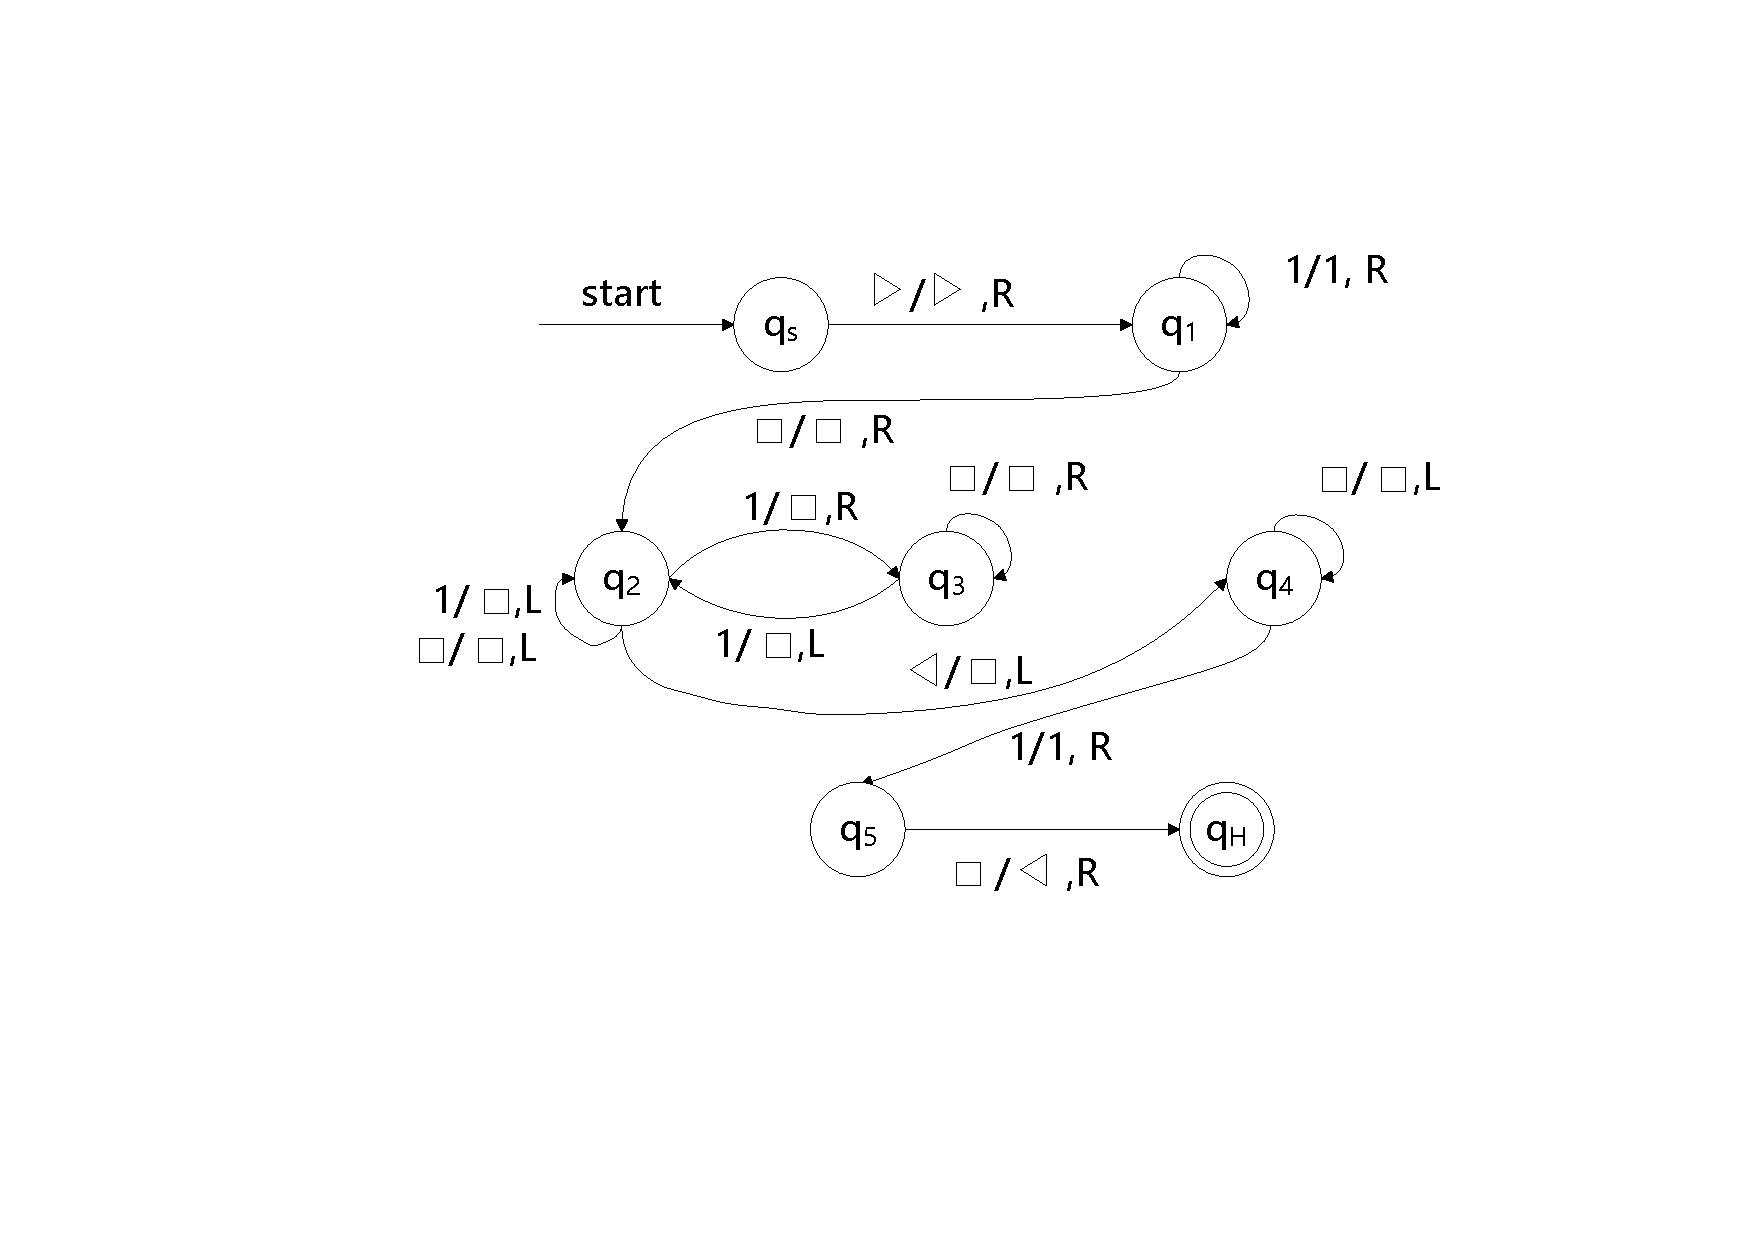
\includegraphics[width=0.8\textwidth]{Fig-transition_diagram.pdf}
            \caption{State transition diagram of this one-tape turing machine to perform function $f(x,y)=x-y$.}\label{fig-state}
        \end{figure}

        (c) The whole process is shown in Figure \ref{fig-process}.
        \begin{figure}
            \centering
            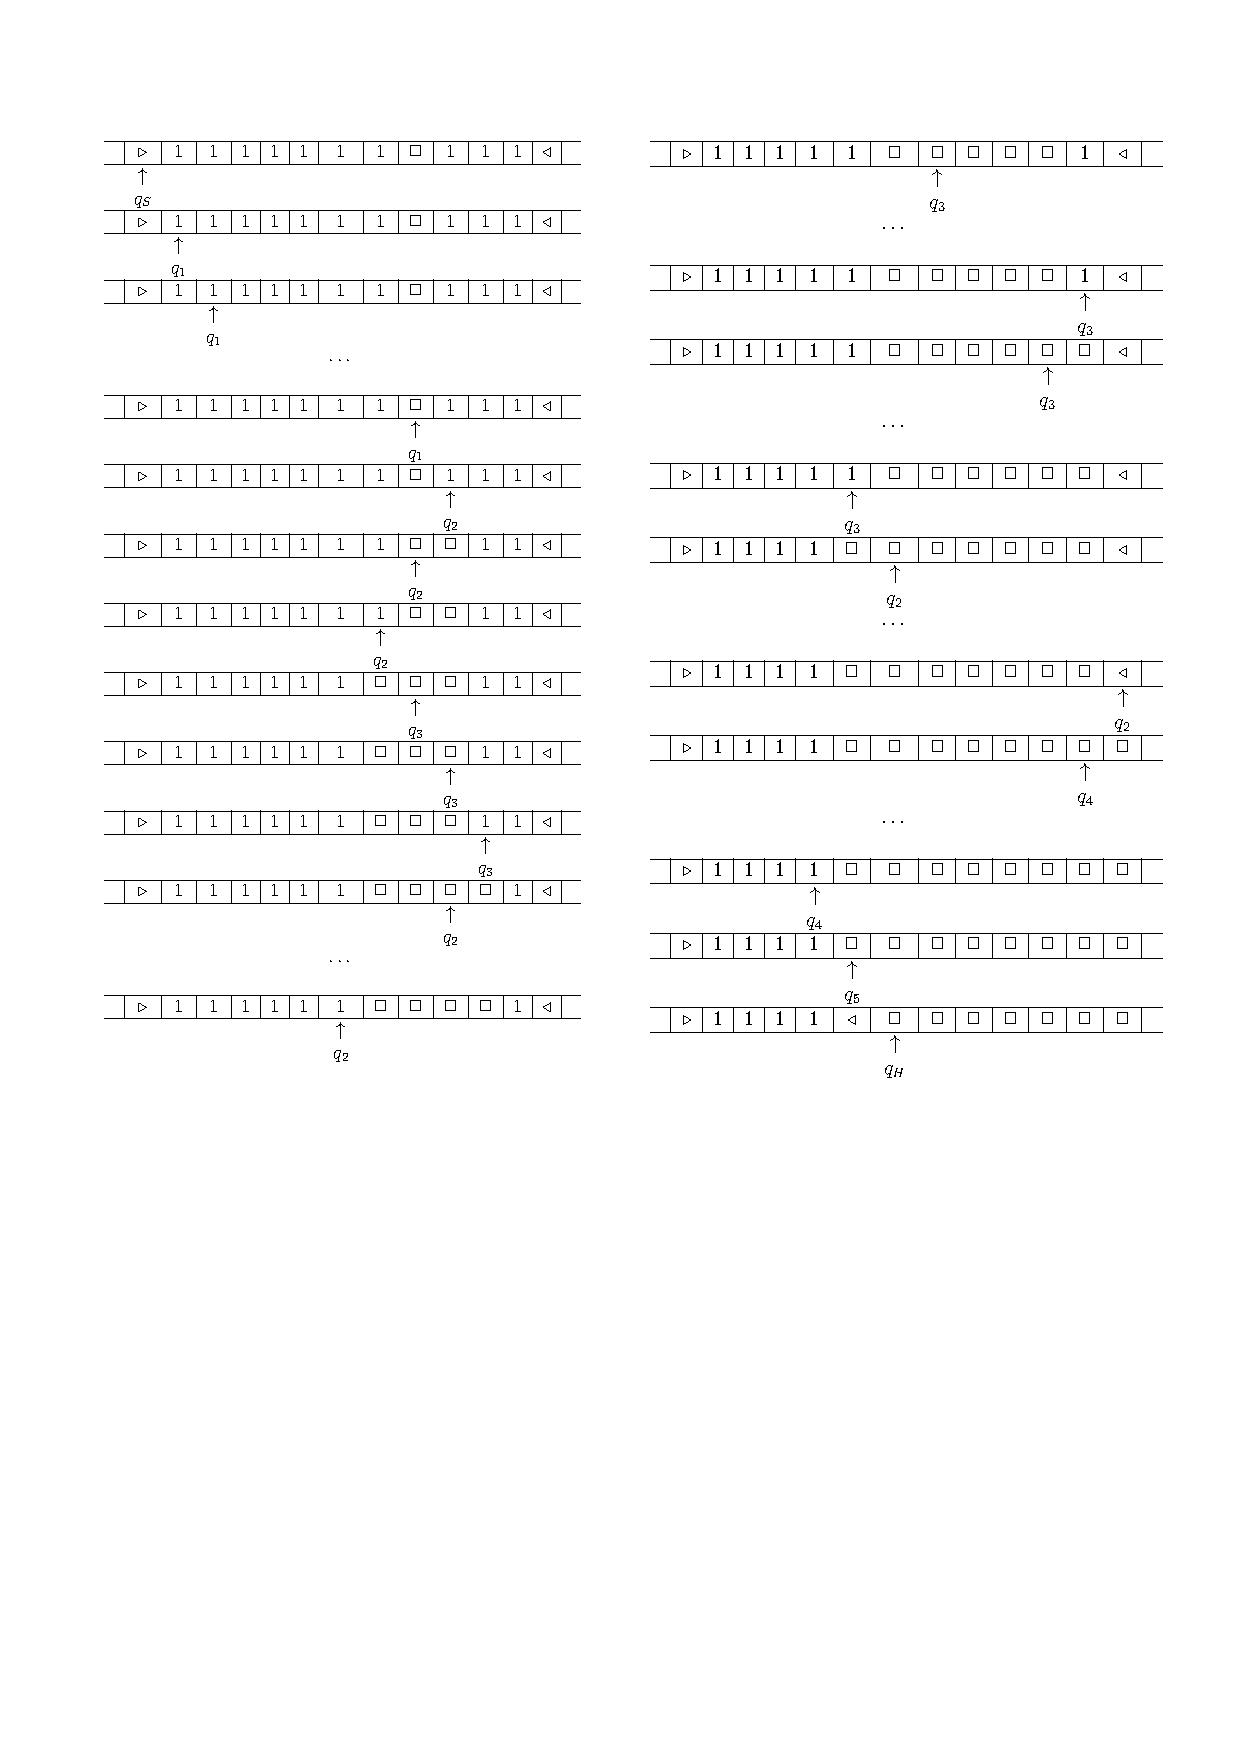
\includegraphics[width=0.9\textwidth]{Fig-whole_process.pdf}
            \caption{The whole process of running TM with input $x=7,y=3$}\label{fig-process}
        \end{figure}
    \end{solution}

    \item
    What is the ``certificate'' and ``certifier'' for the following problems?
    \begin{enumerate}
        \item
        \emph{PARTITION}: Given a finite set $A$ and a size $s(a) \in \mathbb{Z}$ for each $a \in A$, is there a subset $A' \subseteq A$ such that $\sum_{a \in A'}s(a) = \sum_{a \in A-A'}s(a)$ ?

        \item
        \emph{CLIQUE}: Given a graph $G = (V, E)$ and a positive integer $K \leq |V|$, is there a subset $V' \subseteq V$ with $|V'| \geq K$ such that every two vertices in $V'$ are joined by an edge in $E$ ?

        \item
        \emph{ZERO-ONE INTEGER PROGRAMMING}: Given an integer $m \times n$ matrix $A$ and an integer $m$-vector $b$, is there an integer $n$-vector $x$ with elements in the set $\{0, 1\}$ such that $Ax \leq b$ ?
    \end{enumerate}
    \begin{solution}
        (a) \textbf{Certificate} \;A certificate of \emph{PARTITION} problem is a subset $A'\subseteq A$ given in explicit form, such that we can add up $s(a)$ for every $a\in A'$ and $A-A'$.

        \textbf{Certifier} \;A certifier of \emph{PARTITION} problem is the following algorithm:\newline
        \begin{minipage}[t]{0.9\textwidth}
            \begin{algorithm}[H]
              \BlankLine
              \SetKwInOut{Input}{input}
              \SetKwInOut{Output}{output}
              \caption{\emph{PARTITION} Certifier}
              \Input{A finite set $A$, an array of size $s(a)$ for each $a\in A$, an explicit subset $A'\subseteq A$}
              \BlankLine
              $sum1\leftarrow0$, $sum2\leftarrow0$\;
              \ForEach{$a\in A'$}{
                  \If{$a\notin A$}{\Return{false\;}}
              $sum1\leftarrow sum1+s(a)$\;
              }
              \ForEach{$a\in A-A'$}{$sum2\leftarrow sum2+s(a)$\;}
            \eIf{$sum1 = sum2$} {\Return{true\;}}{\Return{false\;}}
            \end{algorithm}
            \end{minipage}
        
            (b)\textbf{Certificate} \;A certificate of \emph{CLIQUE} problem is a subset $V'\subseteq V$ given in explicit form, such that we can check if everytwo vertices in $V'$ are joined by an edge in $E$.

            \textbf{Certifier} \;A certifier of \emph{CLIQUE} problem is the following algorithm:\newline
            \begin{minipage}[t]{0.9\textwidth}
                \begin{algorithm}[H]
                  \BlankLine
                  \SetKwInOut{Input}{input}
                  \SetKwInOut{Output}{output}
                  \caption{\emph{CLIQUE} Certifier}
                  \Input{A graph $G=(V,E)$,an integer $K<|V|$, an explicit subset $V'\subseteq V$}
                  \BlankLine
                  $subsetsize\leftarrow0$\;
                  \ForEach{$v\in V'$}{
                  \If{$v\notin V$}{\Return{false\;}}
              $subsetsize\leftarrow subsetsize+1$\;
              }
                  \If{$subsetsize<K$}{\Return{false\;}}
                  Sort vertices in $V'$ according to some criteria\;
                  \For{$i\leftarrow1$ to $subsetsize$}{
                      \For{$j\leftarrow i$ to $subsetsize$}{
                          \If(\tcp*[l]{$v_i,v_j$ are the i-th and j-th vertices in the sorted $V'$}){$(v_i,v_j)\notin E$} {\Return{false\;}}
                      }
                      }
                \Return{true\;}
                \end{algorithm}
                \end{minipage}

                (c)\textbf{Certificate} \;A certificate of \emph{ZERO-ONE INTEGER PROGRAMMING} problem is an integer $n-$vector $x$ with elements in the set {0,1}.

                \textbf{Certifier} \;A certifier of \emph{ZERO-ONE INTEGER PROGRAMMING} problem is the following algorithm:\newline
                \begin{minipage}[t]{0.9\textwidth}
                    \begin{algorithm}[H]
                      \BlankLine
                      \SetKwInOut{Input}{input}
                      \SetKwInOut{Output}{output}
                      \caption{\emph{ZERO-ONE INTEGER PROGRAMMING} Certifier}
                      \Input{An integer $m\times n$ matrix $A$, an integer $m$-vector $b$, an integer $n-$vector $x$ with elements in the set {0,1}}
                      \BlankLine
                      \For{$i\leftarrow1$ to $n$}{
                          \If{$x[i]\notin\{0,1\}$}{\Return{false\;}}
                      }
                      \For{$i\leftarrow1$ to $m$}{$result[i]\leftarrow0$\;}
                      \For{$i\leftarrow1$ to $m$}{
                          \For{$j\leftarrow1$ to $n$}{
                              $result[i]\leftarrow result[i]+A[i][j]\times x[j]$\;
                          }
                          \If{$result[i]>b[i]$}{\Return{false\;}}
                      }
                    \Return{true\;}
                    \end{algorithm}
                    \end{minipage}
                     
    \end{solution}

    \item
    \emph{SUBSET SUM}: Given a finite set $A$, a size $s(a) \in \mathbb{Z}$ for each $a \in A$ and an integer $B$, is there a subset $A' \subseteq A$ such that $\sum_{a \in A'}s(a) = B$?

    \emph{KNAPSACK}: Given a finite set $A$, a size $s(a) \in \mathbb{Z}$ and a value $v(a) \in \mathbb{Z}$ for each $a \in A$ and integers $B$ and $K$, is there a subset $A' \subseteq A$ such that $\sum_{a \in A'}s(a) \leq B$ and $\sum_{a \in A'}v(a) \geq K$?

    \begin{enumerate}
    \item
    Prove \emph{PARTITION} $\leq_p$ \emph{SUBSET SUM}.

    \item
    Prove \emph{SUBSET SUM} $\leq_p$ \emph{KNAPSACK}.

    \end{enumerate}
    
        \begin{proof}
            (a)Notice that the difference between \emph{PARTITION} and \emph{SUBSET SUM} is that instance of \emph{SUBSET SUM} has an additinal interger $B$ which is irrelavent to $A$. Let us define that $\sum\limits_{a\in A}s(a)=C$,$\sum\limits_{a\in A'}s(a)=D$. We then prove that $A'$ is a partition of $A$ iff $A'$ satisfies \emph{SUBSET SUM} with $B=C-D$.

            ``$\Rightarrow$'': If $A'$ is a partition of $A$, $D=\sum\limits_{a\in A-A'}s(a)=\sum\limits_{a\in A}s(a)-\sum\limits_{a\in A'}s(a)=C-D=B$.

            ``$\Leftarrow$'': If $A'$ satisfies \emph{SUBSET SUM} with $B=C-D$, $D=B=C-D=\sum\limits_{a\in A}s(a)-\sum\limits_{a\in A'}s(a)=\sum\limits_{a\in A-A'}s(a)$. Then $A'$ is a partition of $A$.
            \qed

            (b)Let instance of \emph{KNAPSACK} be that $v(a)=s(a)$, $B=K$. Then for any subset $A'\subseteq A$, it is a yes instance in \emph{SUBSET SUM} iff it is a yes instance in this according \emph{KNAPSACK}.

            ``$\Rightarrow$'': If $A'$ is a yes instance in \emph{SUBSET SUM}, we have $\sum\limits_{a \in A'}s(a) = B=K$. Then we have $\sum\limits_{a \in A'}s(a) \leq B$ and $\sum\limits_{a \in A'}s(a)=\sum\limits_{a \in A'}v(a)\geq K$. Thus $A'$ is a yes instance in \emph{KNAPSACK}.

            ``$\Leftarrow$'': If $A'$ is a yes instance in \emph{KNAPSACK}, we have $\sum\limits_{a \in A'}s(a) \leq B$, $\sum\limits_{a \in A'}s(a)=\sum\limits_{a \in A'}v(a)\geq K=B$, which leads to $\sum\limits_{a \in A'}s(a) = B$. Thus $A'$ is a yes instance in \emph{SUBSET SUM}.
        \end{proof}
    

    \item
    \emph{3-SAT}: Given a set $U$ of variables, a collection $C$ of clauses over $U$ such that each clause $c \in  C$ has $|c| = 3$, is there a satisfying truth assignment for $C$?

    Prove \emph{3-SAT} $\leq_p$ \emph{CLIQUE}.
\begin{proof}
    For every instance $\Phi$ with $n$ variables and $k$ clauses in \emph{3-SAT}, we construct a graph $G$ accordingly and set the integer $K=k$, such that we derive an instance of \emph{CLIQUE}. For each literal in each clause, construct a vertex, and each clause from a 3-vertex gadget. Then connect each vertex to all vertices in other clauses except it negation(s), and the construction is done.
    
    We then prove that answer of the instance in \emph{3-SAT} is yes iff the contructed instance in \emph{CLIQUE} is yes.

    ``$\Rightarrow$'': If $\Phi$ is satisfiable, there exists a set of truth values of variables $x_1,x_2,\cdots,x_n$ s.t. every clause in $\Phi$ is true, i.e. at least one literal in each clause is set to true. Select one true literal in each clause, to form a subset $V'$ of $V$ in the graph, then $|V'|=k\geq K$. And according to the construction process, vertices between different clauses are disconnected only when they are negations to each other, which cannot happen since one literal and its negation cannot be true simultaneously. Thus every two vertices in $V'$ is joined by an edge in $E$, which leads the answer of \emph{CLIQUE} to be yes.

    ``$\Leftarrow$'': If there exists a subset $V'\subseteq V$ with $|V'|\geq K=k$, such that every two vertices in $V'$ is joined by an edge in $E$, then we actually have $|V'|=k$. If $|V'|>k$, then there is at least a clause that has more than one vertex in $V'$. But it contradicts that there does not exist an edge joining two vertices in the same clause. Therefore $|V'|=k$, and each clause contain exactly 1 vertex. We then set the according literals to true, and $\Phi$ is then satisfiable.

    Figure \ref{fig-3sat} is an illustration of the construction.
    \begin{figure}[ht]
        \centering
            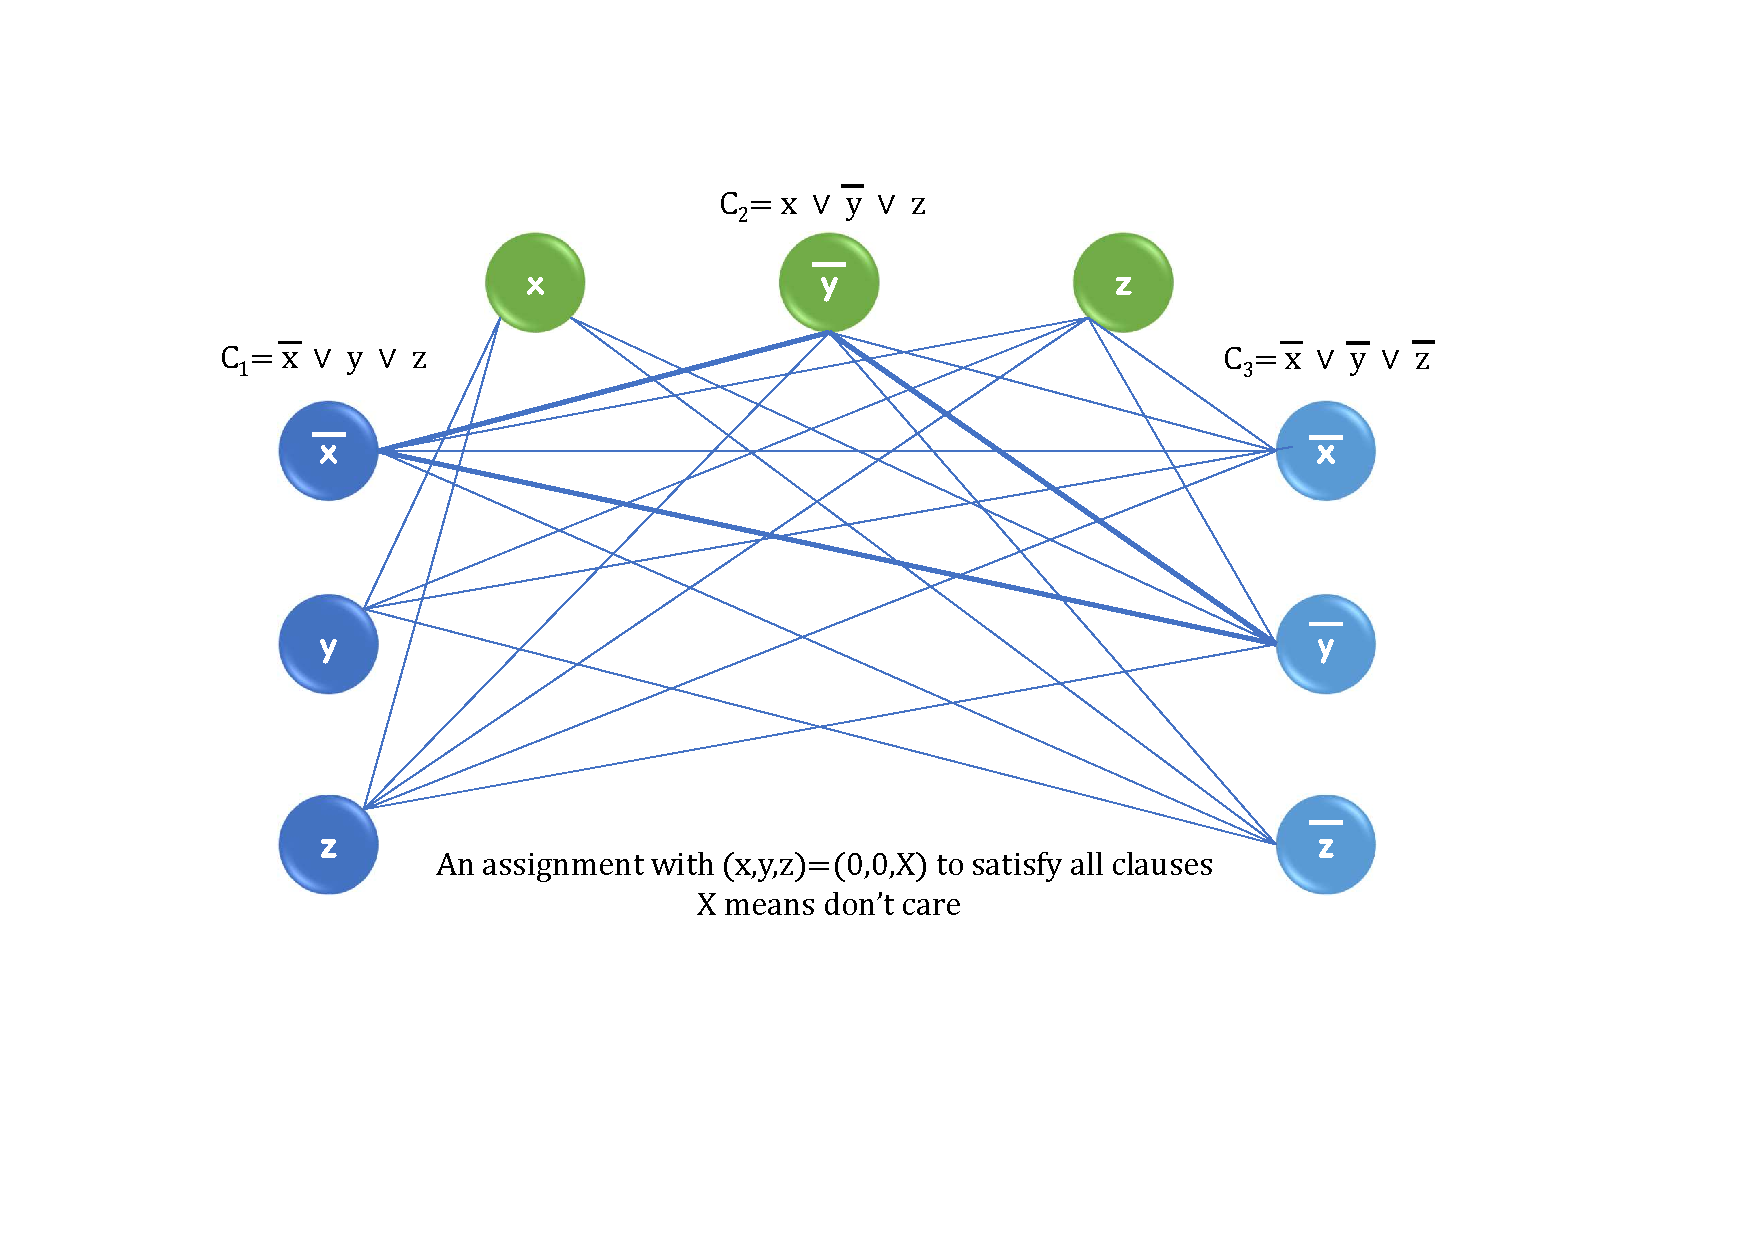
\includegraphics[width=0.6\textwidth]{Fig-3-SAT.pdf}
            \caption{An illustration of the instance constructing process, from \emph{3-SAT} to \emph{CLIQUE}.}\label{fig-3sat}
    \end{figure}
     
\end{proof}

\item Algorithm class is a democratic class. Denote class as a finite set $S$ containing every students. Now students decided to raise a student union $S' \subseteq S$ with $|S'|\leq K$ .\par
As for the members of the union, there are many different opinions. An opinion is a set $S_o\subseteq S$. Note that number of opinions has nothing to do with number of students.\par
The question is whether there exists such student union $S' \subseteq S$ with $|S'|\leq K$, that $S'$ contains at least one element from each opinion. We call this problem \emph{ELECTION} problem, prove that it is NP-complete.


\begin{proof}
    \emph{ELECTION} is actually a famous type of problem called \emph{HITTING-SET}. We give the formalization of this problem: given a finite collection of sets $\{S_1,S_2,\cdots,S_n\}$ and a budget $K$, where $S_o(1\leq o\leq n)$ is a subset of the universal set $S$ , whether there exists a set $S'$ s.t. $\forall o, S_o\cap S'\neq\emptyset$ and $|S'|<K$.

    \textbf{Claim.} \;\emph{VERTEX-COVER} $\leq_P$ \emph{HITTING-SET}.

    Given an undirected graph $G=(V,E)$ and an integer $K$ as an instance of \emph{VERTEX-COVER}, let us construct an instance of \emph{HITTING-SET}. Let vertice $v\in V$ become set elements in $S$, and edge $e_o=(v_i,v_j)\in E$ become a set $S_o=\{v_i,v_j\}$. The integer $K$ becomes the budget of required set. All edges, transformed into sets, then become the collection in \emph{HITTING-SET}. And all vertices become the elements of universal set $S$.

    Then we prove that the answer of the instance in \emph{VERTEX-COVER} is yes iff the contructed instance in \emph{HITTING-SET} is yes.

    ``$\Rightarrow$'': If there exists a vertex cover $V'$ with $|V'|<K$ in graph $G$, then we can pick every vertex in $V'$ to form a set $S'$. Actually $V'=S'$, and $|S'|=|V'|<k$. Since $V'$ is a vertex cover, then for every edge $e_o=(v_i,v_j)\in E$, $v_i\in V'$ or $v_j\in V'$. That means for every set $S_o=\{v_i,v_j\}$, $S'\cap S_o\neq \emptyset$. Thus there exists a hitting set $S'$ for this instance.

    ``$\Leftarrow$'': If there exists a hitting set $S'$ for the given collection $\{S_1,S_2,\cdots,S_n\}$ with respect to the universal set $S$ and a budget $K$, then for every set $S_o=\{v_i,v_j\}$ in the collection, $S'\cap S_o\neq \emptyset$. That is to say, $v_i\in S'$ or $v_j\in S'$. Then for the original edge $e_o=(v_i,v_j)\in E$, $e_o$ is covered by $V'=S'$. Therefore $V'$ is a vertex cover, and $|V'|=|S'|<K$.

    Figure \ref{fig-hitting} is a illustration of \emph{VERTEX-COVER} and \emph{HITTING-SET} with an example.
    \begin{figure}[ht]
        \centering
            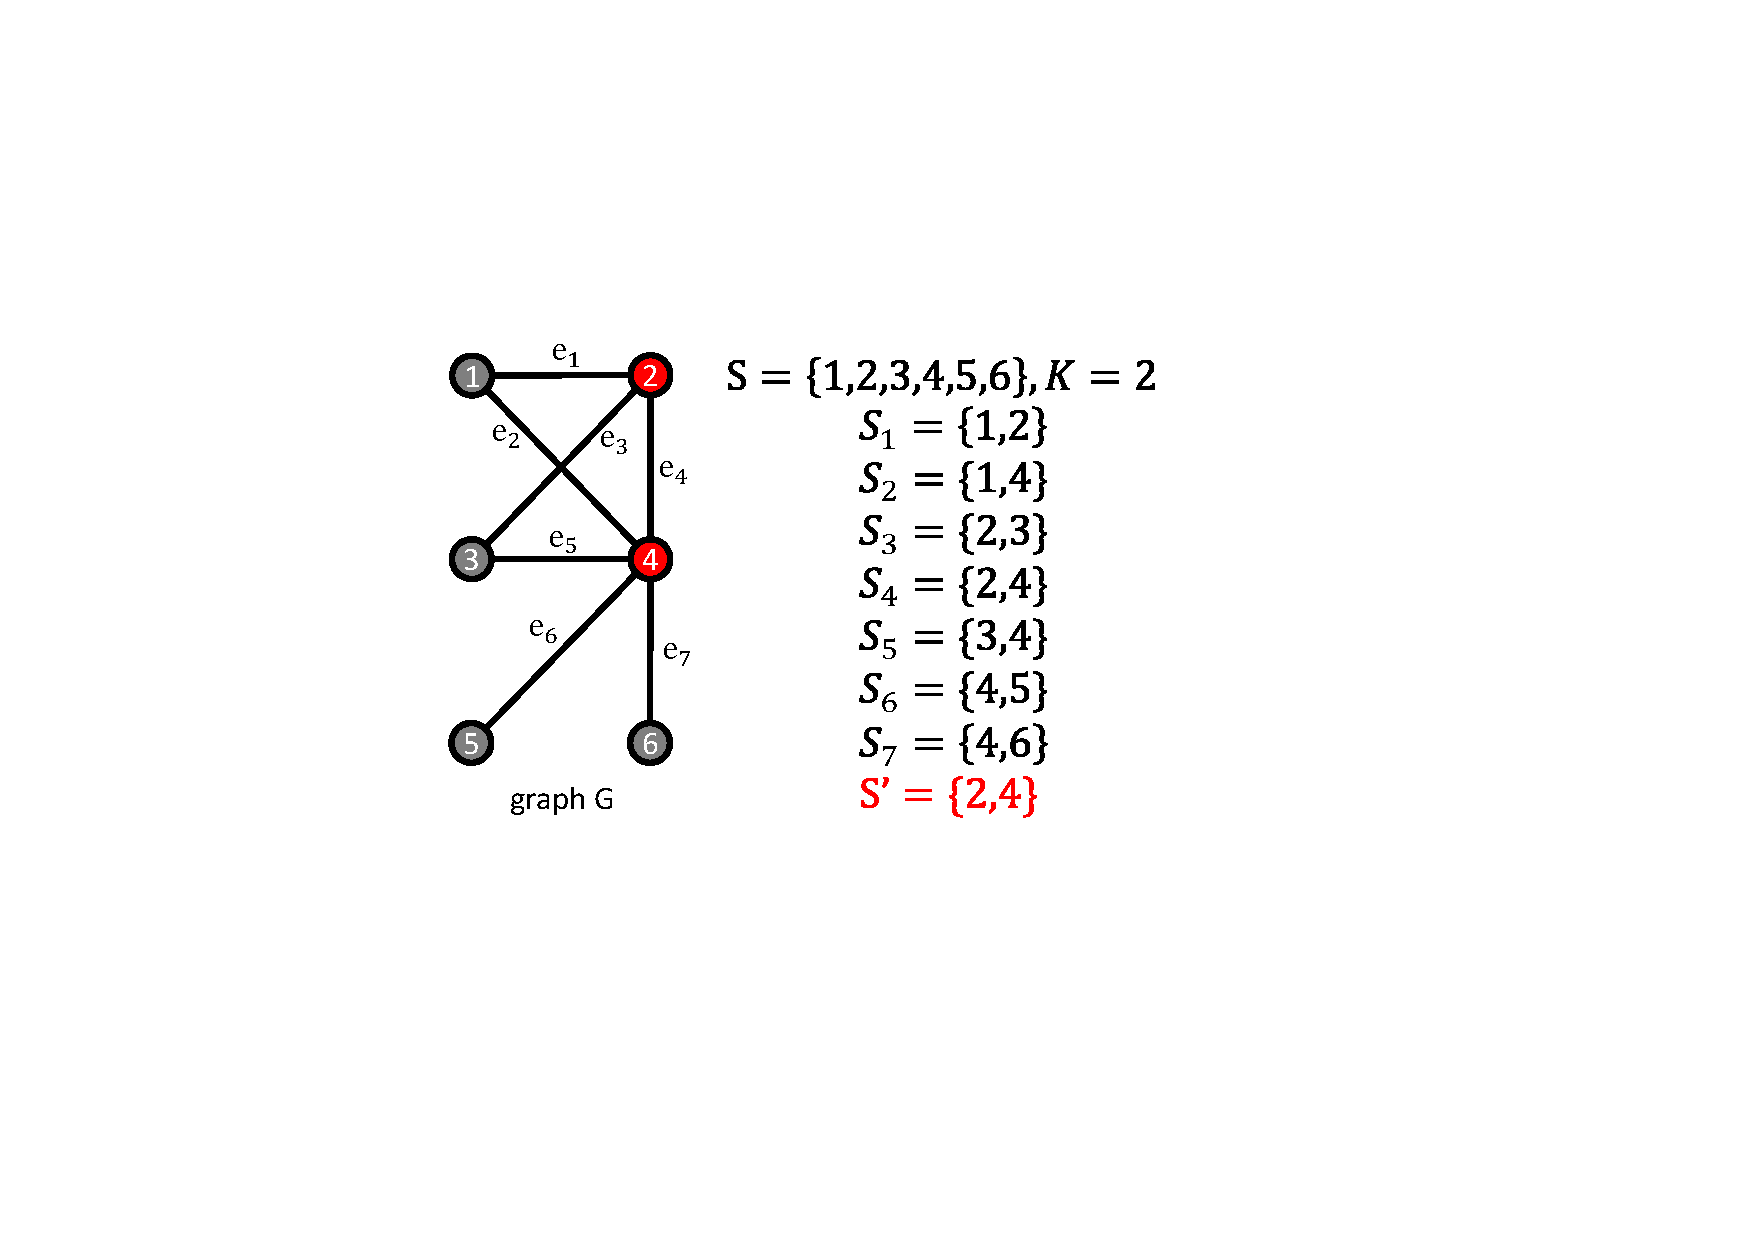
\includegraphics[width=0.6\textwidth]{Fig-hitting_set.pdf}
            \caption{An illustration of the instance constructing process mentioned above.}\label{fig-hitting}
    \end{figure}

    Now that we proved \emph{VERTEX-COVER} $\leq_P$ \emph{HITTING-SET}, and we know that \emph{VERTEX-COVER} is NP-complete, according to the definition of NP-completeness and transitivity of $\leq_P$,  \emph{HITTING-SET}, i.e. \emph{ELECTION} is also NP-complete.
\end{proof}
\end{enumerate}
\vspace{20pt}

\textbf{Remark:} You need to include your .pdf and .tex files in your uploaded .zip file.

%========================================================================
\end{document}
